
\documentclass[letterpaper,hide notes,xcolor={table,svgnames},pdftex]{beamer}
\def\showexamples{t}


%\usepackage[svgnames]{xcolor}

%% Demo talk
%\documentclass[letterpaper,notes=show]{beamer}

\usecolortheme{crane}%seahorse crane
\setbeamertemplate{navigation symbols}{}

\usetheme{MyPittsburgh}
%\usetheme{Frankfurt}

%\usepackage{tipa}

\usepackage{hyperref}
\usepackage{graphicx,xspace}
\usepackage[normalem]{ulem}

\newcommand\SF[1]{$\bigstar$\footnote{SF: #1}}

\usepackage{paratype}
\renewcommand*\familydefault{\sfdefault} %% Only if the base font of the document is to be sans serif
\usepackage[zerostyle=c]{newtxtt}
\usepackage[T1]{fontenc}

\newcounter{tmpnumSlide}
\newcounter{tmpnumNote}

\usepackage{xcolor}
\usepackage{tabu}
\definecolor{light-gray}{gray}{0.75}
\taburulecolor{light-gray}

% old question code
%\newcommand\question[1]{{$\bigstar$ \small \onlySlide{2}{#1}}}
% \newcommand\nquestion[1]{\ifdefined \presentationonly \textcircled{?} \fi \note{\par{\Large \textbf{?}} #1}}
% \newcommand\nanswer[1]{\note{\par{\Large \textbf{A}} #1}}


 \newcommand\mnote[1]{%
   \addtocounter{tmpnumSlide}{1}
   \ifdefined\showcues {~\tiny\fbox{\arabic{tmpnumSlide}}}\fi
   \note{\setlength{\parskip}{1ex}\addtocounter{tmpnumNote}{1}\textbf{\Large \arabic{tmpnumNote}:} {#1\par}}}

\newcommand\mmnote[1]{\note{\setlength{\parskip}{1ex}#1\par}}

%\newcommand\mnote[2][]{\ifdefined\handoutwithnotes {~\tiny\fbox{#1}}\fi
% \note{\setlength{\parskip}{1ex}\textbf{\Large #1:} #2\par}}

%\newcommand\mnote[2][]{{\tiny\fbox{#1}} \note{\setlength{\parskip}{1ex}\textbf{\Large #1:} #2\par}}

\newcommand\mquestion[2]{{~\color{red}\fbox{?}}\note{\setlength{\parskip}{1ex}\par{\Large \textbf{?}} #1} \note{\setlength{\parskip}{1ex}\par{\Large \textbf{A}} #2\par}\ifdefined \presentationonly \pause \fi}

\newcommand\blackboard[1]{%
\ifdefined   \showblackboard
  {#1}
  \else {\begin{center} \fbox{\colorbox{blue!30}{%
         \begin{minipage}{.95\linewidth}%
           \hspace{\stretch{1}} Some space intentionally left blank; done at the blackboard.%
         \end{minipage}}}\end{center}}%
         \fi%
}



%\newcommand\q{\tikz \node[thick,color=black,shape=circle]{?};}
%\newcommand\q{\ifdefined \presentationonly \textcircled{?} \fi}

\usepackage{listings}
\lstset{%
  keywordstyle=\bfseries,
  aboveskip=15pt,
  belowskip=15pt,
  captionpos=b,
  identifierstyle=\ttfamily,
  escapeinside={(*@}{@*)},
  stringstyle=\ttfamiliy,
  frame=lines,
  numbers=left, basicstyle=\scriptsize, numberstyle=\tiny, stepnumber=0, numbersep=2pt}

\usepackage{siunitx}
\newcommand\sius[1]{\num[group-separator = {,}]{#1}\si{\micro\second}}
\newcommand\sims[1]{\num[group-separator = {,}]{#1}\si{\milli\second}}
\newcommand\sins[1]{\num[group-separator = {,}]{#1}\si{\nano\second}}
\sisetup{group-separator = {,}, group-digits = true}

%% -------------------- tikz --------------------
\usepackage{tikz}
\usetikzlibrary{positioning}
\usetikzlibrary{arrows,backgrounds,automata,decorations.shapes,decorations.pathmorphing,decorations.markings,decorations.text}

\tikzstyle{place}=[circle,draw=blue!50,fill=blue!20,thick, inner sep=0pt,minimum size=6mm]
\tikzstyle{transition}=[rectangle,draw=black!50,fill=black!20,thick, inner sep=0pt,minimum size=4mm]

\tikzstyle{block}=[rectangle,draw=black, thick, inner sep=5pt]
\tikzstyle{bullet}=[circle,draw=black, fill=black, thin, inner sep=2pt]

\tikzstyle{pre}=[<-,shorten <=1pt,>=stealth',semithick]
\tikzstyle{post}=[->,shorten >=1pt,>=stealth',semithick]
\tikzstyle{bi}=[<->,shorten >=1pt,shorten <=1pt, >=stealth',semithick]

\tikzstyle{mut}=[-,>=stealth',semithick]

\tikzstyle{treereset}=[dashed,->, shorten >=1pt,>=stealth',thin]

\usepackage{ifmtarg}
\usepackage{xifthen}
\makeatletter
% new counter to now which frame it is within the sequence
\newcounter{multiframecounter}
% initialize buffer for previously used frame title
\gdef\lastframetitle{\textit{undefined}}
% new environment for a multi-frame
\newenvironment{multiframe}[1][]{%
\ifthenelse{\isempty{#1}}{%
% if no frame title was set via optional parameter,
% only increase sequence counter by 1
\addtocounter{multiframecounter}{1}%
}{%
% new frame title has been provided, thus
% reset sequence counter to 1 and buffer frame title for later use
\setcounter{multiframecounter}{1}%
\gdef\lastframetitle{#1}%
}%
% start conventional frame environment and
% automatically set frame title followed by sequence counter
\begin{frame}%
\frametitle{\lastframetitle~{\normalfont(\arabic{multiframecounter})}}%
}{%
\end{frame}%
}
\makeatother

\makeatletter
\newdimen\tu@tmpa%
\newdimen\ydiffl%
\newdimen\xdiffl%
\newcommand\ydiff[2]{%
    \coordinate (tmpnamea) at (#1);%
    \coordinate (tmpnameb) at (#2);%
    \pgfextracty{\tu@tmpa}{\pgfpointanchor{tmpnamea}{center}}%
    \pgfextracty{\ydiffl}{\pgfpointanchor{tmpnameb}{center}}%
    \advance\ydiffl by -\tu@tmpa%
}
\newcommand\xdiff[2]{%
    \coordinate (tmpnamea) at (#1);%
    \coordinate (tmpnameb) at (#2);%
    \pgfextractx{\tu@tmpa}{\pgfpointanchor{tmpnamea}{center}}%
    \pgfextractx{\xdiffl}{\pgfpointanchor{tmpnameb}{center}}%
    \advance\xdiffl by -\tu@tmpa%
}
\makeatother
\newcommand{\copyrightbox}[3][r]{%
\begin{tikzpicture}%
\node[inner sep=0pt,minimum size=2em](ciimage){#2};
\usefont{OT1}{phv}{n}{n}\fontsize{4}{4}\selectfont
\ydiff{ciimage.south}{ciimage.north}
\xdiff{ciimage.west}{ciimage.east}
\ifthenelse{\equal{#1}{r}}{%
\node[inner sep=0pt,right=1ex of ciimage.south east,anchor=north west,rotate=90]%
{\raggedleft\color{black!50}\parbox{\the\ydiffl}{\raggedright{}#3}};%
}{%
\ifthenelse{\equal{#1}{l}}{%
\node[inner sep=0pt,right=1ex of ciimage.south west,anchor=south west,rotate=90]%
{\raggedleft\color{black!50}\parbox{\the\ydiffl}{\raggedright{}#3}};%
}{%
\node[inner sep=0pt,below=1ex of ciimage.south west,anchor=north west]%
{\raggedleft\color{black!50}\parbox{\the\xdiffl}{\raggedright{}#3}};%
}
}
\end{tikzpicture}
}


%% --------------------

%\usepackage[excludeor]{everyhook}
%\PushPreHook{par}{\setbox0=\lastbox\llap{MUH}}\box0}

%\vspace*{\stretch{1}

%\setbox0=\lastbox \llap{\textbullet\enskip}\box0}

\setlength{\parskip}{\fill}

\newcommand\noskips{\setlength{\parskip}{1ex}}
\newcommand\doskips{\setlength{\parskip}{\fill}}

\newcommand\xx{\par\vspace*{\stretch{1}}\par}
\newcommand\xxs{\par\vspace*{2ex}\par}
\newcommand\tuple[1]{\langle #1 \rangle}
\newcommand\code[1]{{\sf \footnotesize #1}}
\newcommand\ex[1]{\uline{Example:} \ifdefined \presentationonly \pause \fi
  \ifdefined\showexamples#1\xspace\else{\uline{\hspace*{2cm}}}\fi}

\newcommand\ceil[1]{\lceil #1 \rceil}


\AtBeginSection[]
{
   \begin{frame}
       \frametitle{Outline}
       \tableofcontents[currentsection]
   \end{frame}
}



\pgfdeclarelayer{edgelayer}
\pgfdeclarelayer{nodelayer}
\pgfsetlayers{edgelayer,nodelayer,main}

\tikzstyle{none}=[inner sep=0pt]
\tikzstyle{rn}=[circle,fill=Red,draw=Black,line width=0.8 pt]
\tikzstyle{gn}=[circle,fill=Lime,draw=Black,line width=0.8 pt]
\tikzstyle{yn}=[circle,fill=Yellow,draw=Black,line width=0.8 pt]
\tikzstyle{empty}=[circle,fill=White,draw=Black]
\tikzstyle{bw} = [rectangle, draw, fill=blue!20, 
    text width=4em, text centered, rounded corners, minimum height=2em]
    
    \newcommand{\CcNote}[1]{% longname
	This work is licensed under the \textit{Creative Commons #1 3.0 License}.%
}
\newcommand{\CcImageBy}[1]{%
	\includegraphics[scale=#1]{creative_commons/cc_by_30.pdf}%
}
\newcommand{\CcImageSa}[1]{%
	\includegraphics[scale=#1]{creative_commons/cc_sa_30.pdf}%
}
\newcommand{\CcImageNc}[1]{%
	\includegraphics[scale=#1]{creative_commons/cc_nc_30.pdf}%
}
\newcommand{\CcGroupBySa}[2]{% zoom, gap
	\CcImageBy{#1}\hspace*{#2}\CcImageNc{#1}\hspace*{#2}\CcImageSa{#1}%
}
\newcommand{\CcLongnameByNcSa}{Attribution-NonCommercial-ShareAlike}


\newenvironment{changemargin}[1]{% 
  \begin{list}{}{% 
    \setlength{\topsep}{0pt}% 
    \setlength{\leftmargin}{#1}% 
    \setlength{\rightmargin}{1em}
    \setlength{\listparindent}{\parindent}% 
    \setlength{\itemindent}{\parindent}% 
    \setlength{\parsep}{\parskip}% 
  }% 
  \item[]}{\end{list}} 




\title{Lecture 29 --- Object-Oriented Programming }

\author{J. Zarnett\\
\texttt{jzarnett@uwaterloo.ca}}
\institute{Department of Electrical and Computer Engineering \\
  University of Waterloo}
\date{\today}

\begin{document}

\begin{frame}
  \titlepage
  
  \begin{center}
  \small{Acknowledgments: W.D. Bishop}
  \end{center}
\end{frame}



\begin{frame}
\frametitle{Structuring a Program}

Up to this point we have organized our program using procedural programming: the use of functions to give us program structure.

We can break down a larger problem into smaller problems, each of which we can accomplish in a re-usable sequence of steps (function).

The painful reality is that most software projects fail.\\
\quad They are often late, unreliable, and/or expensive.

This is because software is extremely complex.\\
\quad We need to manage this complexity if a project is to succeed.\\
\quad Procedural programming is not adequate to the task.

\end{frame}

\begin{frame}
\frametitle{Re-usable Components}

Idea: if an electrical engineer needs a transistor, she does not need to build one from scratch; just go to the bin and use an existing one.

Now take the idea of re-usable components and apply it to software.\\
\quad We've already had re-usable functions, so why not components?

What we'd like is to package up data and functions that manipulate that data into single, self-contained, re-usable unit.

\alert{Objects} are the way of packaging \& managing our data and functions.\\
\quad They are the building blocks of an object-oriented program.

\end{frame}

\begin{frame}
\frametitle{Objects}



An object models a tangible item or some abstract concept:\\
\quad What properties does an object have? What can the object do?

The world is full of ``things'' (objects). Imagine a dog.\\
\quad A dog has characteristics like colour, weight, age...\\
\quad A dog also has behaviours like bark, move, sleep...

To represent a dog in software, create an object that possesses both characteristics (\textbf{data variables}) and behaviours (\textbf{functions}) of a dog.


\end{frame}

\begin{frame}
\frametitle{Object Oriented Programming}

Objects interact with other objects through their functions, and not by manipulating another object's data directly.

Modelling the system as objects and their interactions is known as \alert{Object Oriented Programming}.

C++ supports and encourages this programming paradigm as an approach to designing useful, modular, reusable software systems.

Appropriate use of object oriented programming as a design technique will allow us to create and maintain complex software.

\end{frame}

\begin{frame}
\frametitle{Example: Variable Voltage}
Suppose we want to model a variable voltage source: an electric component that provides several different voltage output levels. 

Let's say it has a selector to choose one of the following levels:\\
\quad Off, 6V, 12V, 18V, and 24V.

What variables will we need to model this?\\
\quad Some constants to hold the possible settings.\\
\quad A variable to represent the current setting.

We also have some functions to represent voltage source behaviour:\\
\quad Increase the voltage by one level.\\
\quad Decrease the voltage by one level.\\
\quad Shut it off.\\


\end{frame}


\begin{frame}
\frametitle{The Blueprints}
We have an idea now about how to model the variable voltage source.\\
\quad Now, to represent that in the program.

Analogy: building ``blueprints'' (architectural plan).

Before a building is built, architects and civil engineers draft a document that describes in detail the structure of the building.

The construction team uses the document when building a structure.\\
\quad It tells them what to do (though not generally how to do it).

\end{frame}

\begin{frame}
\frametitle{Building Blueprints Example}

\begin{center}
	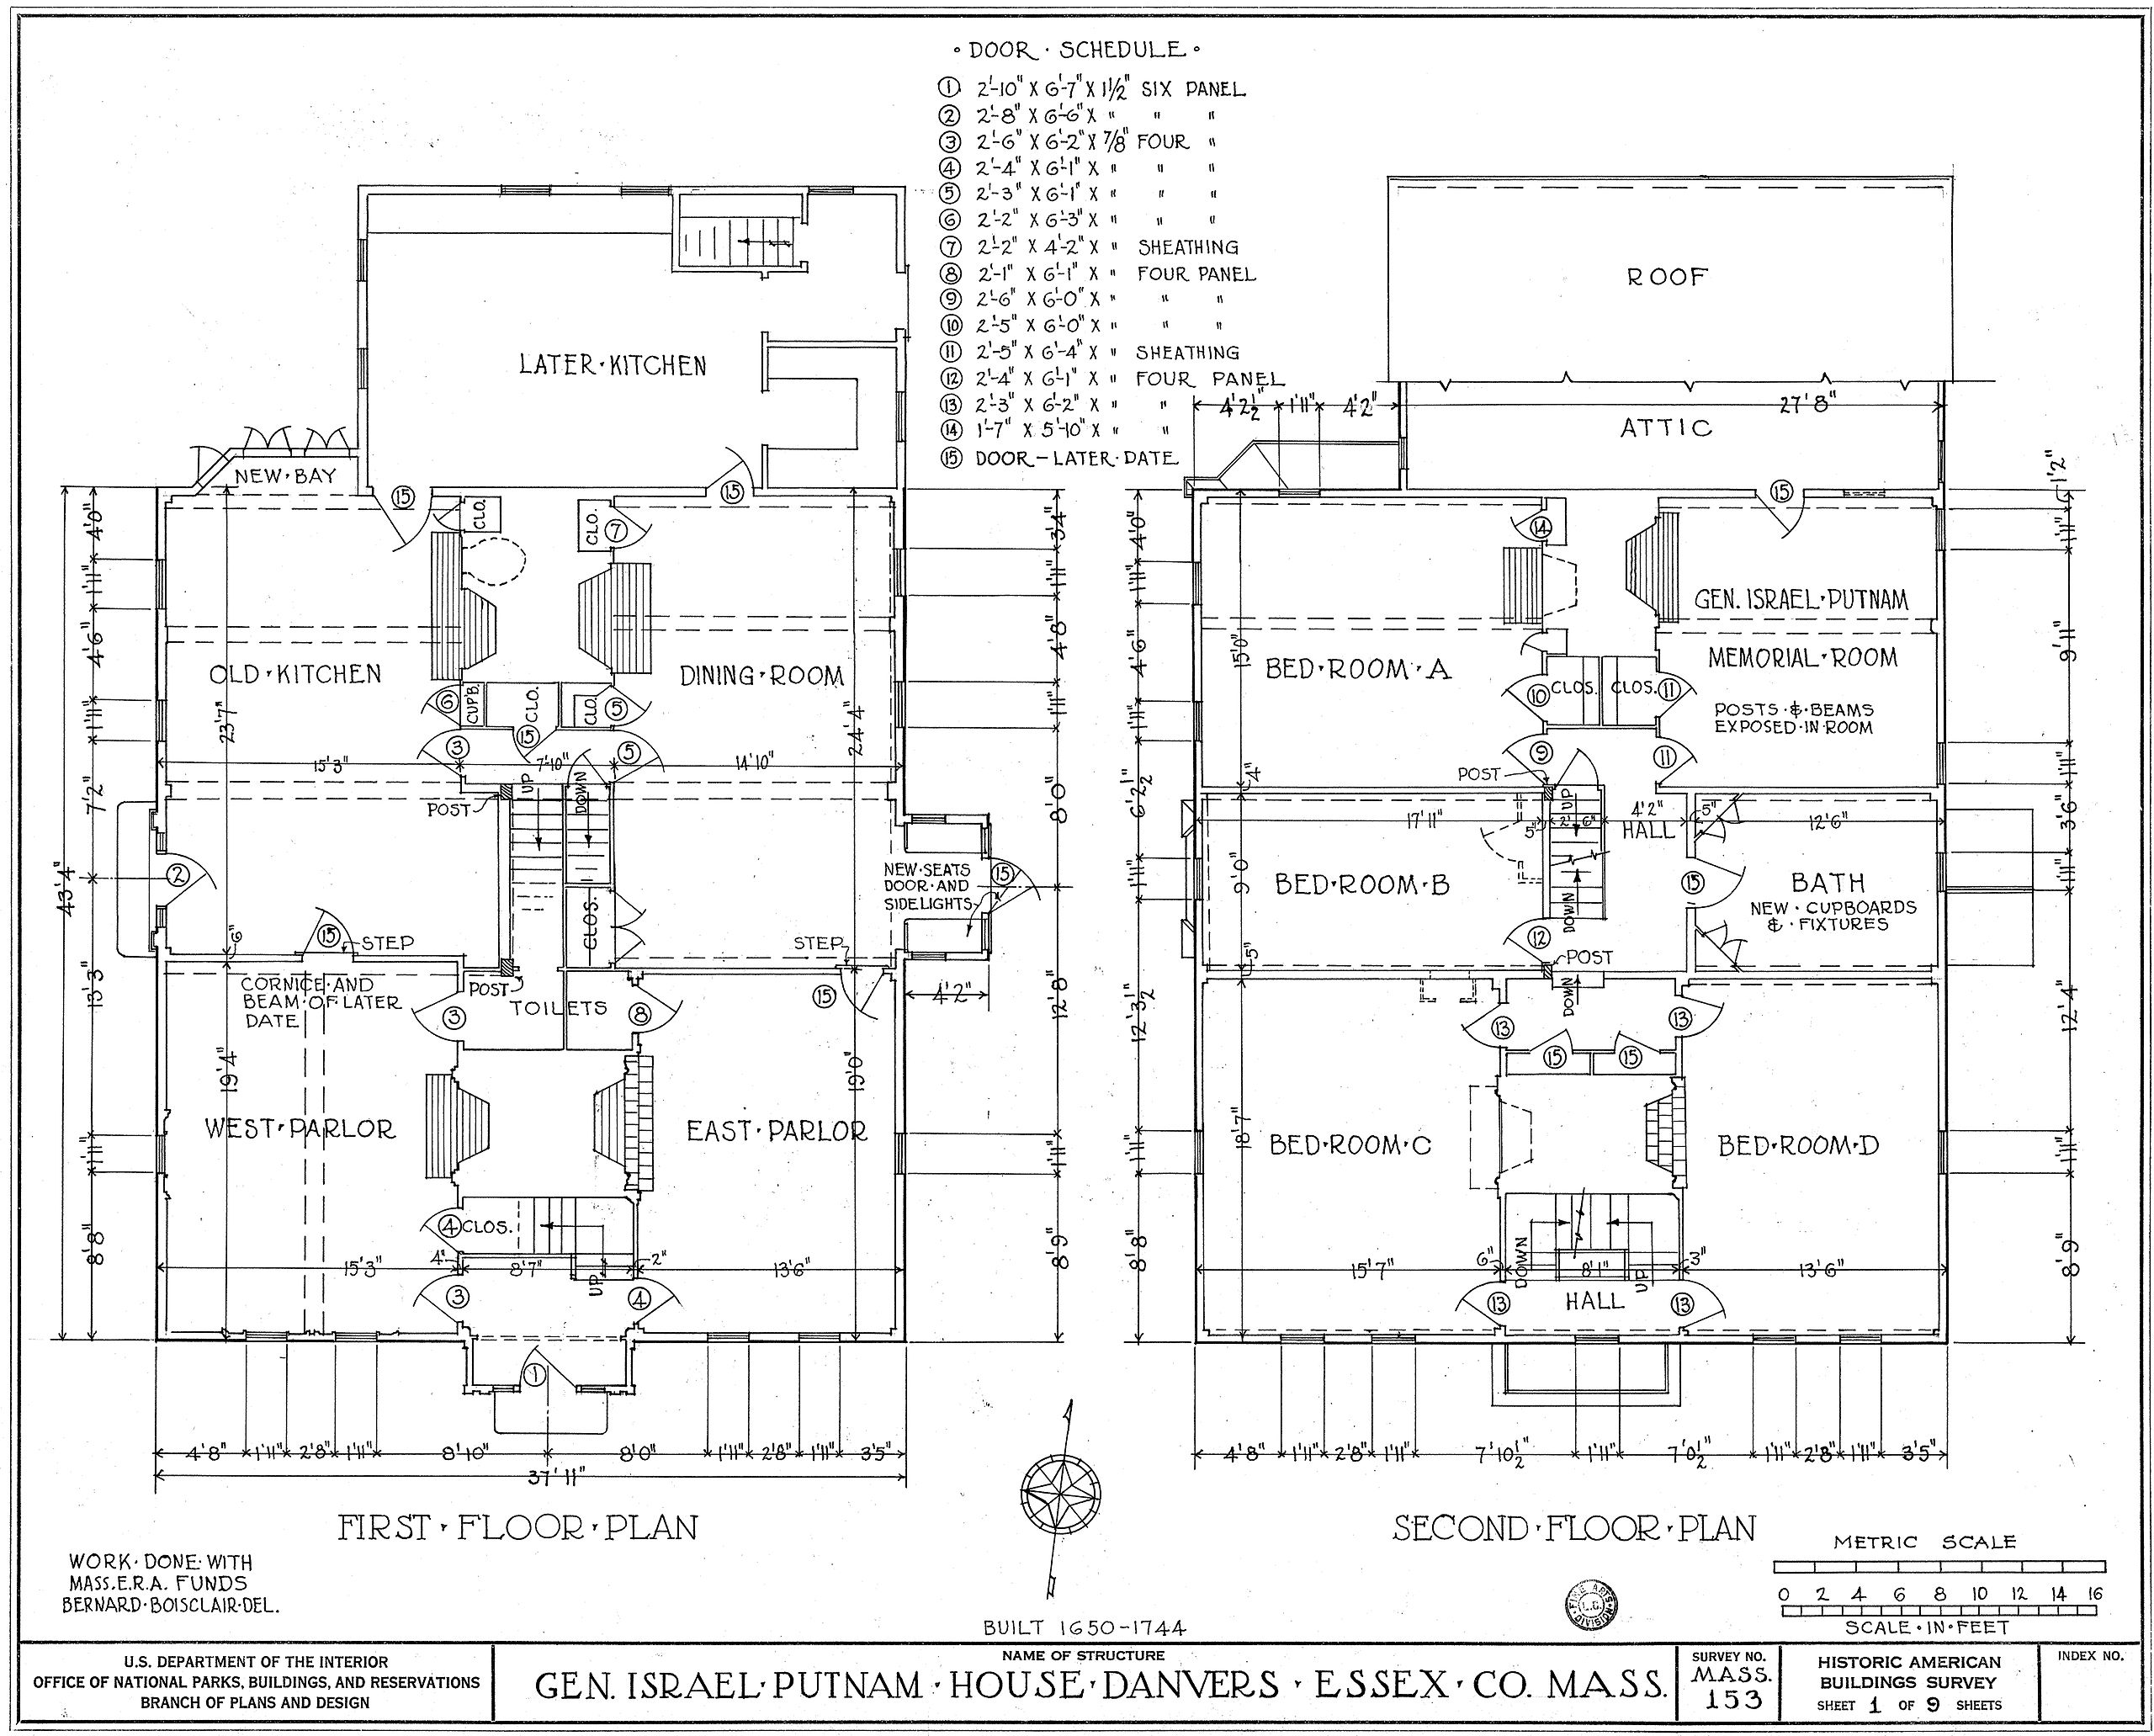
\includegraphics[width=0.85\textwidth]{images/putnamhouse.jpg}
\end{center}
\end{frame}

\begin{frame}
\frametitle{Class Definition}
To tell the system how to build an object, we need to provide it the blueprints for that object.

The blueprints for an object is a \alert{\texttt{class}} definition.\\
\quad This code tells the system how to create an object of that type.

The \texttt{class} definition specifies the variables and methods.

Classes are therefore programmer-defined types.

\end{frame}



\begin{frame}
\frametitle{The Structure}

We've already seen programmer-defined types: the \texttt{struct}.

The \texttt{struct} can contain different variables of different types.

The \texttt{class} is an expanded version of the \texttt{struct}: it contains functions in addition to variables.

The data and functions of an object are referred to as \alert{members}.

Member functions are called \alert{methods}.\\
Member variables are called \alert{fields}.

\end{frame}


\begin{frame}[fragile]
\frametitle{Voltage Source Blueprints}

Let's draw up the blueprints for the voltage source:
{\scriptsize
\begin{verbatim}
class voltage_source
{
  public: 
    int current_voltage;
    int[] voltageLevels = {0, 6, 12, 18, 24};

    void increase_voltage();  
    void decrease_voltage();  
    void turn_off();
};
\end{verbatim}
}

\end{frame}

\begin{frame}
\frametitle{Voltage Source Blueprints Comments}

The previous slide gave the structure for the voltage source we wanted to model: it showed the member fields and methods.

Given this definition, the system now knows how to make a \texttt{voltage\_source} object.

The implementations of the functions are not shown for space reasons, but in defining the class, we would normally fill them in.

Of course, defining the structure of the object is the first step, but if we want to use a \texttt{voltage\_source}, we will need to create one.

\end{frame}


\begin{frame}
\frametitle{Instances}

A specific realization of a class is called an \alert{instance}.\\
\quad A program may create many distinct instances of the same class.

Classes are programmer-defined \textbf{types}, so this is no surprise.\\
\quad We can have many distinct \texttt{double}s in the program.

The process of creating an instance of a class is called \alert{instantiation}.


\end{frame}

\begin{frame}
\frametitle{Classes are Like Structs}
Classes are like structures, so we can use them as types

The declaration
\quad \texttt{voltage\_source source;}\\

  
creates an instance of \texttt{voltage\_source}.

We can then access fields of this instance with the dot operator.

\texttt{source.current\_voltage = 0;}

\end{frame}

\begin{frame}
\frametitle{Car Example}

Let's look at another object example: a car.\\
\quad Data: make, model, year,...\\
\quad Functions: \texttt{honk\_horn(), flash\_lights()}...


Given a \texttt{class Car}, you can make several instances:\\
\quad Toyota Corolla, Chevrolet Corvette, BMW 335i, Volkswagen Jetta...

\end{frame}


\begin{frame}[fragile]
\frametitle{Car Class}

Here's a basic version of the \texttt{Car} class, that looks much like a \texttt{struct}:

{\scriptsize
\begin{verbatim}
class Car
{
    public:
      string make;
      string model;
      int year;
    
      void honk_horn();
      void flash_lights();
      // Other methods not shown for space reasons
};
\end{verbatim}
}

As we learn more about OOP, we will improve this definition to be more useful and consistent with good programming practices.

\end{frame}

\begin{frame}
\frametitle{Using the Dot Operator}

Just like the \texttt{struct}, variables of an instance are accessed using the Dot Operator (\texttt{.}).

\texttt{Car prius;}\\
\quad Declares and instantiates a \texttt{Car} object.

After creation with \texttt{new}, we may access the variables of the instance:\\
\quad \texttt{prius.make  = "Toyota";}\\
\quad \texttt{prius.model = "Prius";}\\
\quad \texttt{prius.year  = 2010;}

\end{frame}



\begin{frame}
\frametitle{Making a Copy of an Instance}

If we want a copy, just using the assignment operator will not do what we want.

We must allocate and create another instance.\\
\quad \texttt{Car prius2;}

To make a copy, create a new instance, and copy the data from the original object to the new instance, one variable at a time.

(In the next lecture, we'll learn a better way to do this.)

\end{frame}

\begin{frame}
\frametitle{Building on the Car Example}

Let's build on the example of the \texttt{Car} class and look at a dealership.

A car dealership has zero or more cars on its parking lot.\\
\quad A good way to implement this might be an array of \texttt{Car} objects.

Just like the \texttt{struct} we can have an array of objects.

When a sales associate wants to find a car to show a customer, they make the lights flash and the horn honk to find the car in the lot.

\end{frame}

\begin{frame}[fragile]
\frametitle{The Car Dealership}

Suppose the parking lot has 42 spaces.

\begin{verbatim}
class Dealership
{
    public:
      int capacity = 42;
      Car[] available_cars[capacity];

      void park( Car new_car, int position );
      void find_car( string make, string model, int year);
      // Other methods and variables not shown
};
\end{verbatim}

What happens if someone tries to park a car in a position that is already occupied?

\end{frame}


\begin{frame}[fragile]
\frametitle{Finding a Specific Car}

Now let's write a method to find a specific car in the lot when we know the make, model, and year.

{\scriptsize
\begin{verbatim}
void Dealership::find_car( string make, string model, int year )
{
    for ( int i = 0; i < capacity; i++ )
    {
        if ( available_cars[i].make == make &&
             available_cars[i].model == model &&
             available_cars[i].year == year)
             {
                 available_cars[i].honk_horn();
                 available_cars[i].flash_lights();
             }
    }
}
\end{verbatim}
}

This function behaves badly if the array of cars is not initialized!

Also, a new piece of syntax: \texttt{::}  -- we will return to this soon.

\end{frame}



\begin{frame}
\frametitle{Use of Methods and Variables}
A common mistake when working with classes is a method call like:\\
\quad \texttt{Car.honk\_horn();}

The compiler identifies this as an error. 

To call the \texttt{honk\_horn()} method, an instance of the class is needed.\\
\quad Which instance of \texttt{Car} do we mean? The Prius? The Jetta?\\
\quad Correct usage: \texttt{prius.honk\_horn();}

Why? These are \alert{instance methods}: they belong to an instance. 


\end{frame}

\begin{frame}[fragile]
\frametitle{The \texttt{static} Keyword}
What does the \texttt{static} keyword mean? The member applies to the type, not an instance.

The keyword \texttt{static} may apply to a field or method.

Consider this very simple class definition:
\begin{verbatim}
class ExampleClass
{
    public:
      int value;
      static int count;
};
\end{verbatim}

\end{frame}

\begin{frame}
\frametitle{Static vs. Instance Members}

In this class, \texttt{value} is an instance member: a new \texttt{int} variable is created whenever a new instance of \texttt{ExampleClass} is created.

But \texttt{count} is a static member: there is only one \texttt{int} variable created, regardless of how many instances of \texttt{ExampleClass} there are.\\
\quad This variable is shared between all instances.\\
\quad It can even be accessed without an instance.

Invalid: \texttt{ExampleClass.value = 1;}\\
Valid: \texttt{ExampleClass.count = 1;}

\end{frame}

\begin{frame}[fragile]
\frametitle{Static vs. Instance Members}
Consider this code:

\begin{verbatim}
ExampleClass* e1 = new ExampleClass( );
ExampleClass* e2 = new ExampleClass( );

e1->value = 7;
e2->value = -8;

e1->count = 2;

cout << "e1 value: " << e1->value << endl;
cout << "e2 value: " << e1->value << endl;
cout << "e1 count: " << e1->count << endl;
cout << "e2 count: " << e2->count << endl;
\end{verbatim}

\end{frame}

\begin{frame}
\frametitle{Static vs. Instance Members}
In the previous slide, we used an instance, \texttt{e1}, to assign the variable \texttt{count}, even though \texttt{count} is \texttt{static}.

This practice is discouraged; if a variable is \texttt{static}, it should be accessed using the \texttt{class} name, not an instance reference.\\
\quad \texttt{ExampleClass.count = 2;}

The compiler may identify using an instance to assign a static variable as a warning.

\end{frame}


\begin{frame}
\frametitle{Static vs. Instance Members}

A \texttt{static} method can make use of static variables and call other static methods, but cannot use instance variables/methods.

Why? Inside the static method, there is no instance to reference.

An instance method can make use of \underline{both} instance and static variables and can call both static and instance methods.

Why? Static methods and variables are always available, as they belong to the type itself.

\end{frame}

\begin{frame}
\frametitle{Static Members}

In the \texttt{voltage\_source} class is an array of different voltage levels:\\
\quad \texttt{int[] voltageLevels = \{0, 6, 12, 18, 24\};}

This is a good candidate to be declared \texttt{static} since the voltage levels will be the same in all of the instances of the class.

\texttt{static int[] voltageLevels = \{0, 6, 12, 18, 24\};}

In general, any constant is likely to be a good candidate to be declared \texttt{static}.

\end{frame}


\end{document}

